\documentclass[11pt,aspectratio=169]{beamer}

\usepackage{booktabs}
\usepackage{array}
\usepackage{multirow}
\usepackage{tikz}
\usepackage{pgfplots}
\usepackage{xcolor}
\usetikzlibrary{positioning,calc,arrows.meta,patterns}
\pgfplotsset{compat=1.18}

\usetheme[titleformat=smallcaps,progressbar=frametitle]{metropolis}
\definecolor{UTburnt}{HTML}{BF5700}
\definecolor{LBJnavy}{HTML}{172A46}
\definecolor{softgray}{HTML}{ECECEC}
\setbeamercolor{alerted text}{fg=UTburnt}
\setbeamercolor{frametitle}{bg=LBJnavy,fg=white}
\setbeamercolor{progress bar}{fg=UTburnt,bg=gray!25}
\setbeamertemplate{navigation symbols}{}

\author{Sergio I. Garc\'ia-R\'ios}
\title{Exploratory Data Analysis}
\subtitle{Comparing Groups and Relationships}
\institute{PA 311N: Data Analysis for Public Policy\\LBJ School of Public Affairs}
\date{Fall 2026}

\newcommand{\yourturn}[1]{%
\begin{center}
\begin{minipage}{0.88\textwidth}
\begin{alertblock}{Your Turn}
#1
\end{alertblock}
\end{minipage}
\end{center}}

\begin{document}
\maketitle

\begin{frame}{Where we left off}
Last time we focused on exploring \alert{one variable at a time}.

\vspace{0.6em}
\begin{columns}[T]
\begin{column}{0.46\textwidth}
\textbf{Categorical variables}
\begin{itemize}
  \item Counts
  \item Proportions
  \item Bar plots
\end{itemize}
\end{column}
\begin{column}{0.46\textwidth}
\textbf{Quantitative variables}
\begin{itemize}
  \item Histograms
  \item Mean and median
  \item Spread and unusual values
\end{itemize}
\end{column}
\end{columns}

\vspace{0.8em}
Today we ask a harder question: \alert{How do variables relate to one another?}
\end{frame}

\begin{frame}{The basic EDA question}
Suppose we observe a difference or a pattern.

\begin{center}
\Large Is it \alert{real}, \alert{important}, or just an artifact of how we looked at the data?
\end{center}

\vspace{0.6em}
Exploratory data analysis helps us:
\begin{itemize}
  \item compare groups;
  \item identify relationships;
  \item find unusual observations;
  \item discover alternative explanations;
  \item decide what to investigate next.
\end{itemize}
\end{frame}

\begin{frame}{Start with the types of variables}
The plot we choose depends on the variables we are comparing.

\vspace{0.5em}
\begin{center}
\renewcommand{\arraystretch}{1.35}
\begin{tabular}{lll}
\toprule
\textbf{Variable 1} & \textbf{Variable 2} & \textbf{Useful display} \\
\midrule
Categorical & Categorical & Two-way table / segmented bar plot \\
Categorical & Quantitative & Side-by-side boxplots \\
Quantitative & Quantitative & Scatterplot \\
\bottomrule
\end{tabular}
\end{center}

\vspace{0.7em}
\alert{First identify the variable types. Then choose the tool.}
\end{frame}

\section{Two categorical variables}

\begin{frame}{Two categorical variables: compare proportions}
Imagine a survey asking whether respondents support a housing policy.

\begin{center}
\renewcommand{\arraystretch}{1.25}
\begin{tabular}{lrrr}
\toprule
 & Support & Oppose & Total \\
\midrule
Renters & 72 & 28 & 100 \\
Homeowners & 54 & 46 & 100 \\
\bottomrule
\end{tabular}
\end{center}

\yourturn{Which group is more supportive? What quantity did you compare?}
\end{frame}

\begin{frame}{Counts are not always enough}
Now suppose the group sizes differ.

\begin{center}
\renewcommand{\arraystretch}{1.25}
\begin{tabular}{lrrr}
\toprule
 & Support & Oppose & Total \\
\midrule
Renters & 144 & 56 & 200 \\
Homeowners & 81 & 69 & 150 \\
\bottomrule
\end{tabular}
\end{center}

\vspace{0.5em}
Comparing raw counts can mislead when group sizes differ.

\begin{center}
\alert{Compare conditional proportions: support \emph{within} each group.}
\end{center}
\end{frame}

\begin{frame}{A segmented bar plot makes the comparison visible}
\begin{center}
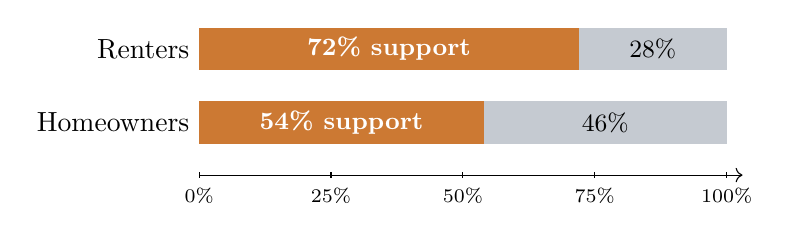
\begin{tikzpicture}[x=6.7cm,y=0.72cm]
  % renters
  \fill[UTburnt!80] (0,2.0) rectangle (0.72,2.75);
  \fill[LBJnavy!25] (0.72,2.0) rectangle (1,2.75);
  \node[left] at (0,2.38) {Renters};
  \node[white,font=\small\bfseries] at (0.36,2.38) {72\% support};
  \node[font=\small] at (0.86,2.38) {28\%};
  % homeowners
  \fill[UTburnt!80] (0,0.7) rectangle (0.54,1.45);
  \fill[LBJnavy!25] (0.54,0.7) rectangle (1,1.45);
  \node[left] at (0,1.08) {Homeowners};
  \node[white,font=\small\bfseries] at (0.27,1.08) {54\% support};
  \node[font=\small] at (0.77,1.08) {46\%};
  % axis
  \draw[->] (0,0.15) -- (1.03,0.15);
  \foreach \x/\lab in {0/0,0.25/25,0.5/50,0.75/75,1/100}
    \draw (\x,0.1)--(\x,0.2) node[below=2pt,font=\scriptsize]{\lab\%};
\end{tikzpicture}
\end{center}

\vspace{0.5em}
Segmented bars emphasize \alert{composition within groups}.

\yourturn{What is the substantive difference between the two groups?}
\end{frame}

\begin{frame}{Ask the right percentage question}
For a two-way table, there is more than one possible percentage.

\vspace{0.6em}
\begin{itemize}
  \item What percent of \textbf{renters} support the policy?
  \item What percent of \textbf{supporters} are renters?
\end{itemize}

These are \alert{different questions} with different denominators.

\vspace{0.8em}
\begin{center}
\Large Always ask: \textbf{``Percent of what?''}
\end{center}
\end{frame}

\section{One categorical and one quantitative variable}

\begin{frame}{Comparing a quantitative outcome across groups}
Suppose we want to compare rent burden across three metropolitan areas.

\vspace{0.5em}
\begin{itemize}
  \item Outcome: percent of household income spent on rent
  \item Group: metropolitan area
\end{itemize}

A single mean for each city can hide important differences in the distributions.

\vspace{0.6em}
\begin{center}
\alert{We want to compare center, spread, and unusual observations.}
\end{center}
\end{frame}

\begin{frame}{Side-by-side boxplots}
\begin{center}
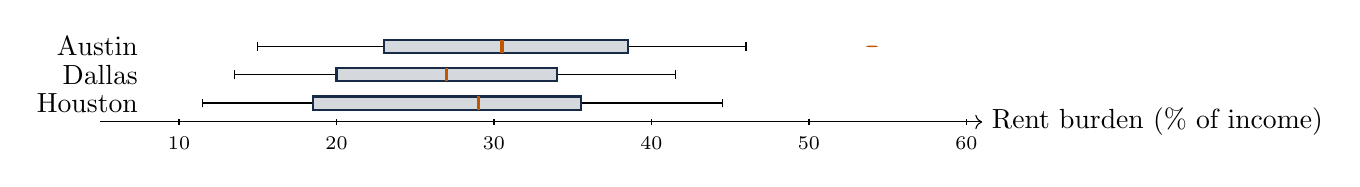
\begin{tikzpicture}[x=1cm,y=0.12cm]
  \draw[->] (0,0) -- (11.2,0) node[right] {Rent burden (\% of income)};
  \foreach \x/\lab in {1/10,3/20,5/30,7/40,9/50,11/60}
    \draw (\x,-0.35)--(\x,0.35) node[below=3pt,font=\scriptsize]{\lab};

  % Austin y=8
  \node[left] at (0.6,8) {Austin};
  \draw (2.0,8)--(8.2,8);
  \draw (2.0,7.55)--(2.0,8.45); \draw (8.2,7.55)--(8.2,8.45);
  \fill[LBJnavy!18] (3.6,7.3) rectangle (6.7,8.7);
  \draw[LBJnavy,thick] (3.6,7.3) rectangle (6.7,8.7);
  \draw[UTburnt,very thick] (5.1,7.3)--(5.1,8.7);
  \fill[UTburnt] (9.8,8) circle (0.08);

  % Dallas y=5
  \node[left] at (0.6,5) {Dallas};
  \draw (1.7,5)--(7.3,5);
  \draw (1.7,4.55)--(1.7,5.45); \draw (7.3,4.55)--(7.3,5.45);
  \fill[LBJnavy!18] (3.0,4.3) rectangle (5.8,5.7);
  \draw[LBJnavy,thick] (3.0,4.3) rectangle (5.8,5.7);
  \draw[UTburnt,very thick] (4.4,4.3)--(4.4,5.7);

  % Houston y=2
  \node[left] at (0.6,2) {Houston};
  \draw (1.3,2)--(7.9,2);
  \draw (1.3,1.55)--(1.3,2.45); \draw (7.9,1.55)--(7.9,2.45);
  \fill[LBJnavy!18] (2.7,1.3) rectangle (6.1,2.7);
  \draw[LBJnavy,thick] (2.7,1.3) rectangle (6.1,2.7);
  \draw[UTburnt,very thick] (4.8,1.3)--(4.8,2.7);
\end{tikzpicture}
\end{center}

\small Illustrative distributions.

\yourturn{Which metro has the highest typical rent burden? Which shows the most spread? Where is the unusual observation?}
\end{frame}

\begin{frame}{What a boxplot summarizes}
\begin{columns}[T]
\begin{column}{0.52\textwidth}
\begin{itemize}
  \item Median
  \item First and third quartiles
  \item Interquartile range (IQR)
  \item Potential outliers
\end{itemize}
\end{column}
\begin{column}{0.44\textwidth}
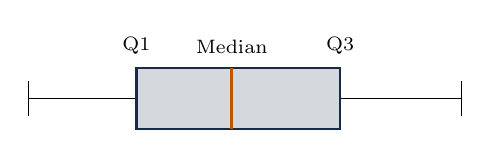
\begin{tikzpicture}[x=0.55cm,y=0.55cm]
  \draw (0,2)--(10,2);
  \draw (0,1.6)--(0,2.4); \draw (10,1.6)--(10,2.4);
  \fill[LBJnavy!18] (2.5,1.3) rectangle (7.2,2.7);
  \draw[LBJnavy,thick] (2.5,1.3) rectangle (7.2,2.7);
  \draw[UTburnt,very thick] (4.7,1.3)--(4.7,2.7);
  \node[above,font=\scriptsize] at (2.5,2.8) {Q1};
  \node[above,font=\scriptsize] at (4.7,2.8) {Median};
  \node[above,font=\scriptsize] at (7.2,2.8) {Q3};
\end{tikzpicture}
\end{column}
\end{columns}

\vspace{0.6em}
Boxplots are especially useful for comparing the \alert{same outcome across several groups}.
\end{frame}

\begin{frame}{Do not reduce every comparison to the mean}
Two groups can have the same average but very different distributions.

\vspace{0.5em}
\begin{center}
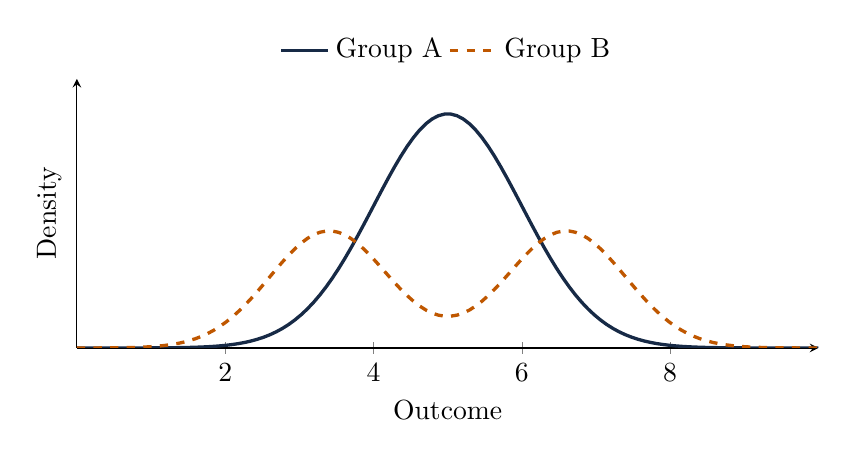
\begin{tikzpicture}
\begin{axis}[
  width=11cm,height=5cm,
  xmin=0,xmax=10,ymin=0,ymax=0.46,
  axis lines=left,
  xlabel={Outcome},ylabel={Density},
  ytick=\empty,
  xtick={2,4,6,8},
  legend style={draw=none,at={(0.5,1.02)},anchor=south,legend columns=2},
]
\addplot[LBJnavy,very thick,domain=0:10,samples=120] {0.40*exp(-0.5*((x-5)/1.0)^2)};
\addlegendentry{Group A}
\addplot[UTburnt,very thick,dashed,domain=0:10,samples=120] {0.20*exp(-0.5*((x-3.4)/0.8)^2)+0.20*exp(-0.5*((x-6.6)/0.8)^2)};
\addlegendentry{Group B}
\end{axis}
\end{tikzpicture}
\end{center}

Same center does not mean same distribution.
\end{frame}

\section{Two quantitative variables}

\begin{frame}{Two quantitative variables: use a scatterplot}
Suppose we compare county median income with the uninsured rate.

\begin{center}
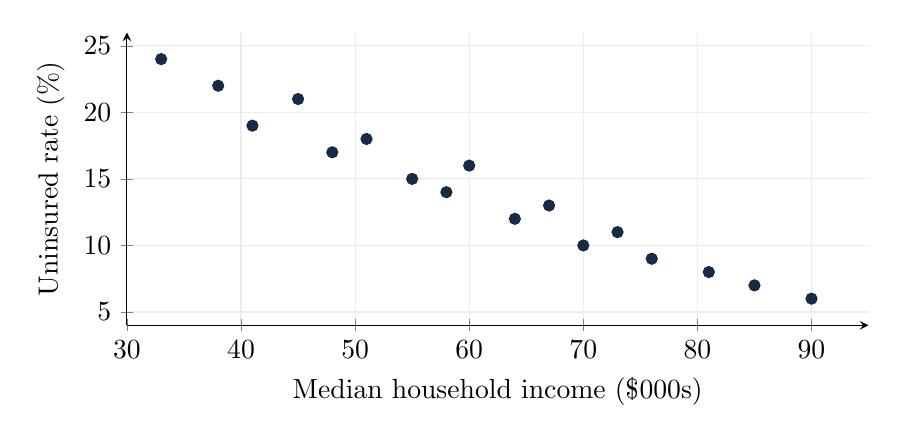
\begin{tikzpicture}
\begin{axis}[
  width=11cm,height=5.3cm,
  xmin=30,xmax=95,ymin=4,ymax=26,
  xlabel={Median household income (\$000s)},
  ylabel={Uninsured rate (\%)},
  axis lines=left,
  grid=major,
  grid style={gray!15}
]
\addplot[only marks,mark=*,mark size=2.0pt,LBJnavy] coordinates {
(33,24)(38,22)(41,19)(45,21)(48,17)(51,18)(55,15)(58,14)(60,16)(64,12)(67,13)(70,10)(73,11)(76,9)(81,8)(85,7)(90,6)
};
\end{axis}
\end{tikzpicture}
\end{center}

\small Illustrative county-level data.
\end{frame}

\begin{frame}{Describe a scatterplot before explaining it}
When looking at two quantitative variables, describe:

\begin{enumerate}
  \item \alert{Direction}: positive, negative, or no clear direction
  \item \alert{Form}: roughly linear, curved, clustered
  \item \alert{Strength}: tight or diffuse pattern
  \item \alert{Unusual observations}: points that do not fit the pattern
\end{enumerate}

\vspace{0.6em}
Only after describing the pattern should we ask \textbf{why} it might exist.
\end{frame}

\begin{frame}{Association is not explanation}
Suppose higher-income counties tend to have lower uninsured rates.

That is an \alert{association}.

It does \textbf{not} tell us by itself whether higher income causes lower uninsured rates.

\vspace{0.6em}
Other differences may matter:
\begin{itemize}
  \item age composition;
  \item employment structure;
  \item state policy;
  \item urbanization;
  \item access to public programs.
\end{itemize}
\end{frame}

\begin{frame}{A third variable can change the story}
A variable related to both the explanatory variable and the outcome can distort the relationship we see.

\vspace{0.8em}
\begin{center}
\Large This is the idea of a \alert{confounding variable}.
\end{center}

\vspace{0.7em}
EDA should make us ask:

\begin{center}
\textbf{What happens when we break the data into meaningful groups?}
\end{center}
\end{frame}

\section{Simpson's paradox}

\begin{frame}{An apparent admissions gap}
UC Berkeley graduate admissions, 1973:

\begin{center}
\renewcommand{\arraystretch}{1.2}
\begin{tabular}{lrrr}
\toprule
 & Admitted & Rejected & Admit rate \\
\midrule
Men & 1,198 & 1,493 & 44.5\% \\
Women & 557 & 1,278 & 30.4\% \\
\bottomrule
\end{tabular}
\end{center}

\vspace{0.6em}
\yourturn{Looking only at this table, what conclusion might you draw? What information is missing?}
\vspace{-0.2em}
{\tiny Source: \texttt{datasets::UCBAdmissions}; Bickel, Hammel, and O\'Connell (1975).}
\end{frame}

\begin{frame}{Now compare within departments}
\begin{center}
\scriptsize
\renewcommand{\arraystretch}{1.16}
\begin{tabular}{lrrrr}
\toprule
 & \multicolumn{2}{c}{Men} & \multicolumn{2}{c}{Women} \\
\cmidrule(lr){2-3}\cmidrule(lr){4-5}
Dept. & Admitted & Rate & Admitted & Rate \\
\midrule
A & 512 & 62.1\% & 89 & 82.4\% \\
B & 353 & 63.0\% & 17 & 68.0\% \\
C & 120 & 36.9\% & 202 & 34.1\% \\
D & 138 & 33.1\% & 131 & 34.9\% \\
E & 53 & 27.7\% & 94 & 23.9\% \\
F & 22 & 5.9\% & 24 & 7.0\% \\
\bottomrule
\end{tabular}
\end{center}

\vspace{0.4em}
The aggregate difference changes substantially once department is considered.
\end{frame}

\begin{frame}{Why did the aggregate pattern appear?}
Applicants were distributed differently across departments with very different admission rates.

\vspace{0.6em}
\begin{itemize}
  \item Women applied more often to departments with lower overall admission rates.
  \item Men applied more often to departments with higher overall admission rates.
\end{itemize}

\vspace{0.7em}
\begin{center}
\alert{The aggregate relationship was partly a product of composition.}
\end{center}

\vspace{0.6em}
This is a classic example of \textbf{Simpson's paradox}: a relationship can weaken, disappear, or reverse after conditioning on another variable.
\end{frame}

\begin{frame}{The lesson is bigger than Simpson's paradox}
Whenever you compare groups, ask:

\begin{itemize}
  \item Are the groups composed differently?
  \item Is there an important third variable?
  \item Would the pattern change within subgroups?
  \item Are we comparing like with like?
\end{itemize}

\vspace{0.8em}
\begin{center}
\Large \alert{Good EDA is skeptical of the first pattern you see.}
\end{center}
\end{frame}

\section{Patterns and uncertainty}

\begin{frame}{Observed differences are not automatically meaningful}
Imagine 52\% support in one sample and 48\% in another.

\vspace{0.6em}
Is the difference:
\begin{itemize}
  \item a stable population difference?
  \item random sample-to-sample variation?
  \item a consequence of measurement or selection?
\end{itemize}

\vspace{0.6em}
EDA tells us \alert{what we observed}.

Inference will later help us evaluate \alert{how much uncertainty surrounds it}.
\end{frame}

\begin{frame}{Description, association, causation}
Keep these three questions separate.

\vspace{0.5em}
\begin{center}
\renewcommand{\arraystretch}{1.35}
\begin{tabular}{p{0.24\textwidth}p{0.60\textwidth}}
\toprule
\textbf{Question} & \textbf{Example} \\
\midrule
Description & What is the uninsured rate? \\
Association & Do uninsured rates differ by income? \\
Causation & Would changing a policy reduce the uninsured rate? \\
\bottomrule
\end{tabular}
\end{center}

\vspace{0.6em}
EDA is essential for all three, but \alert{EDA alone does not establish causation}.
\end{frame}

\section{A practical workflow}

\begin{frame}{A practical EDA workflow}
\begin{enumerate}
  \item Identify the substantive question.
  \item Identify the unit of observation and variable types.
  \item Examine each variable on its own.
  \item Compare variables using an appropriate display.
  \item Look for unusual observations and subgroup differences.
  \item Consider alternative explanations.
  \item Write a descriptive conclusion that matches the evidence.
\end{enumerate}
\end{frame}

\begin{frame}{From question to plot}
\begin{center}
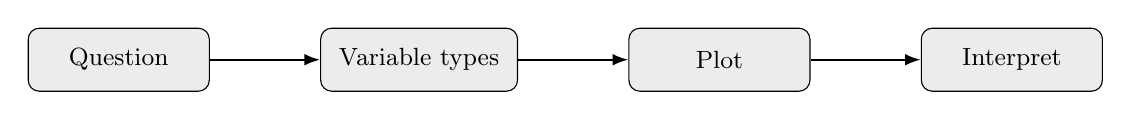
\begin{tikzpicture}[node distance=1.25cm and 1.4cm, every node/.style={font=\small}]
\node[draw,rounded corners,fill=softgray,minimum width=2.3cm,minimum height=0.8cm] (q) {Question};
\node[draw,rounded corners,fill=softgray,right=of q,minimum width=2.5cm,minimum height=0.8cm] (v) {Variable types};
\node[draw,rounded corners,fill=softgray,right=of v,minimum width=2.3cm,minimum height=0.8cm] (p) {Plot};
\node[draw,rounded corners,fill=softgray,right=of p,minimum width=2.3cm,minimum height=0.8cm] (i) {Interpret};
\draw[-{Latex[length=2mm]},thick] (q)--(v);
\draw[-{Latex[length=2mm]},thick] (v)--(p);
\draw[-{Latex[length=2mm]},thick] (p)--(i);
\end{tikzpicture}
\end{center}

\vspace{1em}
\begin{center}
\renewcommand{\arraystretch}{1.28}
\begin{tabular}{lll}
\toprule
Cat. + Cat. & $\rightarrow$ & segmented bar / two-way table \\
Cat. + Quant. & $\rightarrow$ & side-by-side boxplots \\
Quant. + Quant. & $\rightarrow$ & scatterplot \\
\bottomrule
\end{tabular}
\end{center}
\end{frame}

\begin{frame}{Your turn: choose the display}
For each question, choose a useful visualization.

\begin{enumerate}
  \item Does policy support differ by party identification?
  \item Do rents differ across neighborhoods?
  \item Is county income related to the uninsured rate?
\end{enumerate}

\vspace{0.8em}
\pause
\begin{center}
\alert{1. Segmented bar plot \qquad 2. Side-by-side boxplots \qquad 3. Scatterplot}
\end{center}
\end{frame}

\begin{frame}{What you should be able to do now}
Given a substantive question, you should be able to:

\begin{itemize}
  \item identify the relevant variables and their types;
  \item choose an appropriate visualization;
  \item describe patterns in terms of center, spread, direction, and unusual observations;
  \item compare groups using proportions rather than raw counts when appropriate;
  \item recognize that a third variable can change an apparent relationship;
  \item avoid making causal claims from descriptive patterns alone.
\end{itemize}
\end{frame}

\begin{frame}[standout]
\Large Explore first.\\[0.4em]
\normalsize Then decide what the data can actually support.
\end{frame}

\end{document}
